\documentclass[letterpaper, 10pt, journal]{IEEEtran}
\usepackage{graphicx}
\usepackage{float}
\usepackage{listings}
\usepackage{color}
\usepackage{multirow}
\usepackage[table,xcdraw]{xcolor}
\usepackage[justification=centering]{caption}
% Paquete para referenciar figuras
\usepackage{nameref}
\graphicspath{ {./Images/} }
% Paquetes para las funciones matematicas
\usepackage{amsmath}
\usepackage{amssymb}

\usepackage[justification=centering]{caption}
\lstset{frame=tb,
  language=Java,
  aboveskip=3mm,
  belowskip=3mm,
  showstringspaces=false,
  columns=flexible,
  basicstyle={\small\ttfamily},
  numbers=none,
  numberstyle=\tiny\color{gray},
  keywordstyle=\color{blue},
  commentstyle=\color{dkgreen},
  stringstyle=\color{mauve},
  breaklines=true,
  breakatwhitespace=true,
  tabsize=3
}

\begin{document}
\title{Tarea 1 - Reporte de \LaTeX{}  }
\author{Kathy~Brenes~Guerrero, Barnum~Castillo~Barquero

~\IEEEmembership{
    \begin{center}
        Maestr\'ia en Ciencias de la Computaci\'on, Introducci\'on a la Investigaci\'on, ITCR
    \end{center}
}}% <-this % stops a space

% The paper headers
\markboth{Instituto Tecnol\'ogico de Costa Rica, Introducci\'on a la Investigaci\'on, Agosto~2018}%
{Shell \MakeLowercase{\textit{et al.}}: Tarea 1 - Reporte de \LaTeX{}  }
\maketitle

\section{Introducci\'on}
El siguiente reporte detalla la historia, y conceptos b\'asicos y principales del lenguaje de programaci\'on \LaTeX{}. Cada una de las siguientes secciones incorpora un ejemplo aplicado de los t\'erminos comentados con la intenci\'on de educar al lector sobre el uso de \LaTeX{} como herramienta para estructurar documentos de \'indole cient\'ifica y de gran complejidad.

\section{Historia de \LaTeX{}  }
TeX es el programa original de composici\'on matem\'atica desarrollado alrededor de 1980 por Donald Knuth  para la composici\'on tipogr\'afica digital de alta calidad.\cite{[3]} TEX es un lenguaje de bajo nivel con el que las computadoras pueden trabajar, pero a la mayor\'ia de las personas les resultar\'ia dif\'icil usarlo; entonces \LaTeX{} ha sido desarrollado para hacerlo m\'as f\'acil.\cite{[2]}. Se pronuncia como \textquotedblleft{}tecnolog\'{i}a\textquotedblright{} como en alta tecnolog\'ia. La X es la letra griega chi, que hace que el sonido \textquotedblleft{}ch\textquotedblright{} aparezca al final de \textquotedblleft{}tech\textquotedblright{}. En la documentaci\'on original para TeX, hay mucha discusi\'on acerca de \textquotedblleft{}pegar\textquotedblright{} objetos juntos y de \textquotedblleft{}estirar\textquotedblright{} el espacio entre los objetos que componen una p\'agina. \cite{[3]} El l\'{a}tex es un producto natural pegajoso que forma la base del caucho, por lo que se puede inferir que ese es el motivo de la palabra \LaTeX{}. 

\LaTeX{} no es un intento de sonar en franc\'{e}s; probablemente no sea La TeX, o \textquotedblleft{}The TeX\textquotedblright{}. La raz\'{o}n de la divertida alternancia de letras may\'{u}sculas y min\'{u}sculas es que TeX y \LaTeX{}, cuando se escriben correctamente de esta manera, son todas letras may\'{u}sculas, pero en diferentes tama\~{n}os y alturas, unas por encima y por debajo de la l\'{\i}nea base y alternando may\'{u}sculas y min\'{u}sculas. \cite{[3]}

\LaTeX{} est\'{a} construido sobre TeX y fue escrito a principios de la d\'{e}cada de 1980 por Leslie Lamport. Tiene m\'{a}s funciones de alto nivel integradas que TeX, por lo que tiende a ser m\'{a}s f\'{a}cil de usar.
\LaTeX{} se cre\'o para facilitar la producci\'on de libros y art\'iculos de uso general dentro de TeX. Debido a que \LaTeX{} es una extensi\'on del sistema de composici\'on tipogr\'afica TeX, tiene la capacidad de TeX para compilar documentos t\'ecnicos que contienen ecuaciones matem\'aticas complejas. Esta caracter\'istica hizo que \LaTeX{} fuera popular entre cient\'ificos e ingenieros. \cite{[1]}

La producci\'on de un documento \LaTeX{} comienza con un archivo de texto que contiene estructuras etiquetadas con c\'odigos especiales \LaTeX{}, utilizados para indicar c\'omo se dise\~nar\'a el texto. Cuando el archivo se ejecuta a trav\'es de un procesador \LaTeX{}, se producen p\'aginas de composici\'on tipogr\'afica. Debido a que la composici\'on tipogr\'afica \LaTeX{} requiere envolver el texto en c\'odigos inform\'aticos complicados, por lo que tiene una curva de aprendizaje bastante empinada. Aunque ahora hay programas de software que ayudan a automatizar la creaci\'on de documentos \LaTeX{}, un conocimiento pr\'actico de \LaTeX{} sigue siendo deseable para este tipo de composici\'on tipogr\'afica.

\LaTeX{} fue uno de los primeros programas de composici\'on tipogr\'afica capaz de producir ecuaciones matem\'aticas complejas. Con los a\~nos se ha utilizado para componer muchas revistas cient\'ificas, matem\'aticas y de ingenier\'{i}a; la American Mathematical Society (AMS) incluso tiene su propio conjunto de extensiones llamado AMS-LaTeX; pero los programas de autoedici\'on como Quark Inc. de Quark Inc. y FrameMaker de Adobe Systems Incorporated se volvieron m\'as capaces de producir expresiones matem\'aticas complejas, por lo que \LaTeX{} se hizo menos popular.\cite{[1]}

La versi\'on actual de \LaTeX{} es \LaTeX{} 2e. \cite{[2]}

\section{Usos acad\'emicos, extensi\'on, importancia}
\LaTeX{} es un sistema de preparaci\'on de documentos para producir documentos de aspecto profesional, no es un procesador de textos. Es particularmente adecuado para producir documentos largos y estructurados, y es muy bueno para escribir ecuaciones. Est\'a disponible como software libre para la mayor\'ia de los sistemas operativos.

Si est\'a acostumbrado a producir documentos con Microsoft Word, encontrar\'a que \LaTeX{} es un estilo de trabajo muy diferente. En Microsoft Word \textquotedblleft{}lo que ves es lo que obtienes\textquotedblright{} (WYSIWYG), esto significa que puedes ver c\'omo ser\'a el documento final mientras escribe. Cuando trabaje de esta manera, probablemente realice cambios en la apariencia del documento (como espacios entre l\'ineas, encabezados, saltos de p\'agina). Con \LaTeX{} es el caso contrario, esto le permite concentrarse en el contenido m\'as all\'a de la apariencia. \LaTeX{} se basa en la idea de que es mejor dejar el diseño del documento a los dise\~{a}dores y permitir que los autores contin\'{u}en con la escritura del contenido. \cite{[2]}

Un documento \LaTeX{} es un archivo de texto sin formato con una extensi\'on de archivo .tex. Se puede escribir en un editor de texto simple como el Bloc de notas, pero la mayor\'ia de las personas encuentran que es m\'as f\'acil usar un editor de \LaTeX{} dedicado. Mientras escribe, marque la estructura del documento (t\'itulo, cap\'itulos, subt\'itulos, listas, etc.) con etiquetas. Cuando finaliza el documento, comp\'ilelo; esto significa convertirlo a otro formato. \cite{[2]} Existen varios formatos de salida diferentes, pero probablemente el m\'as \'util sea Portable Document Format (PDF), que aparece tal como se imprimir\'a y se puede transferir f\'acilmente entre computadoras. \cite{[2]}

\textbf{Implementaciones de \LaTeX{}}
\begin{enumerate}
    \item Composici\'on de art\'iculos de revistas, informes t\'ecnicos, libros y presentaciones de diapositivas.
    \item Control sobre documentos grandes que contienen secciones, referencias cruzadas, tablas y figuras.
    \item Composici\'on tipogr\'afica de f\'ormulas matem\'aticas complejas.
    \item Composici\'on tipogr\'afica avanzada de las matem\'aticas con AMS-LaTeX.
    \item Generaci\'on autom\'atica de bibliograf\'ias e \'indices.
    \item Composici\'on tipogr\'afica multiling\"ue.
    \item Inclusi\'on de obras de arte, y color de proceso o mancha.
    \item Utilizando fuentes PostScript o Metafont.
\end{enumerate}

\subsection{Tipo de archivo}
Los archivos \LaTeX{} no son tan self-contained como, por ejemplo, los documentos de Word. Sin embargo, sus tama\~{n}os de archivo son generalmente m\'{a}s peque\~{n}os. Aqu\'{\i} hay una descripci\'{o}n muy b\'{a}sica.

Un archivo fuente \LaTeX{} debe recibir la extensi\'{o}n .tex, \'este corresponde a un documento de texto y puede ser editado con Notepad o SimpleText. El archivo fuente \LaTeX{} contiene el texto de sus documentos m\'{a}s los comandos que indican c\'{o}mo deben formatearse el texto y las ecuaciones, de esta manera, es un poco como c\'{o}digo de computadora o HTML sin formato.

Los archivos fuente \LaTeX{} deben ser procesados por un programa que sepa c\'{o}mo interpretar los diversos comandos integrados en ellos. En una PC puede descargar varias implementaciones de \LaTeX{} como: MiKTeX; en Macintosh puede usar OzTeX; en una m\'{a}quina UNIX deber\'{\i}a ser capaz de instalar l\'{a}tex. Me referir\'{e} gen\'{e}ricamente a estos programas como \LaTeX{}. Tenga en cuenta que el programa Texify puede ser el programa real que se utiliza para procesar un documento.

Cuando \LaTeX{} procesa un archivo fuente como example.tex, \'este crea un archivo llamado example.dvi (DeVice Independent). DVI es un formato anterior a .pdf, y pretende ser lo que dice, un formato que pueden manejar muchos dispositivos diferentes (plataformas de computadora). Cada plataforma de computadora tiene sus propios programas que pueden ver (algunos dicen vista previa) archivos .dvi. En una PC, MikTex viene con YAP (Yet Another Previewer); en Macintosh, una vista previa dvi est\'{a} integrada en OzTeX; y en una m\'{a}quina UNIX, generalmente puede encontrar un programa llamado xdvi. \LaTeX{} tambi\'{e}n produce un archivo .aux y .log, del cual no tenemos que preocuparnos ahora.

La progresi\'on habitual al componer un documento en \LaTeX{} es escribir el archivo .tex usando un editor de texto, luego procesarlo usando \LaTeX{} y, finalmente, ver el resultado de .dvi usando un reproductor de vista previa. \'Esta sucesi\'on se debe principalmente al hecho de que \LaTeX{} se desarroll\'o en una plataforma UNIX, en la cual los programas tienden a estructurarse as\'i porque es m\'as modular y m\'as f\'acil tener a muchas personas involucradas en el desarrollo, en lugar de una sola empresa monol\'itica de desarrollo de software. 

No puede enviar un archivo .dvi a una impresora. La mayor\'{\i}a de las impresoras aceptan entradas PostScript (.ps). En una PC, puede abrir el archivo .dvi con YAP para imprimirlo. Con OzTeX, puede seleccionar Archivo, Imprimir. En UNIX, primero utiliza un programa como dvips para convertir el archivo .dvi a un archivo .ps, luego env\'{\i}a el archivo .ps a la impresora usando un comando como lp file.ps.

Finalmente, una vez que crea un documento \LaTeX{}, puede compartir el resultado electr\'{o}nicamente con otros, ya sea por correo electr\'{o}nico como un archivo adjunto o publicarlo en una p\'{a}gina web. Las personas que no usan TeX o LaTeX generalmente no tienen instaladas las previsualizaciones .dvi y .ps, pero a menudo tienen Adobe Acrobat Reader, que puede leer y visualizar archivos .pdf (Portable Document Format). En una PC, probablemente use pdflatex para procesar el c\'{o}digo fuente de \LaTeX{} y producir salida .pdf autom\'{a}ticamente o puede usar un convertidor de DVI a PDF como dvipdfm, que viene con MiKTeX. 
En un Macintosh, puede usar Adobe Distiller (use Sherlock para buscarlo, luego ejec\'{u}telo) para convertir un archivo .ps en un archivo .pdf, luego use Acrobat Reader para verlo. En UNIX, puede usar dvipdf o ps2pdf. La principal desventaja de producir directamente salida .pdf de l\'{a}tex al editar su archivo fuente .tex es que una vez que Adobe Reader tiene un archivo abierto, \LaTeX{} no puede modificar el archivo en el disco. Las previsualizaciones dvi como YAP no tienen este problema.

\section{Estilos de documento }
\begin{lstlisting}
    \documentclass[options]{article}
    Preamble (for LaTeX commands only)
    \begin{document}
    Document text (text with embedded LaTeX commands)
    \end{document}
\end{lstlisting}

Mediante el comando \textbf{document class} se determina el dise\~{n}o y la estructura general del documento. Adem\'{a}s la opci\'on \textbf{article} permite establecer espec\'ificamente los usos y las propiedades que se van a desarrollar, otras clases com\'{u}nmente utilizadas son:

\subsection{Article} 
Como su nombre indica, destinada a escribir art\'{\i}culos. Esto significa documentos relativamente cortos que no contienen cap\'{\i}tulos o partes, solo secciones, subsecciones, etc. Como una de las clases base, el formato es bastante b\'{a}sico. Sin embargo, como la clase de art\'{\i}culo proporciona la funci\'{o}n b\'{a}sica que la mayor\'{\i}a de la gente espera de \LaTeX{}, a menudo se usa con modificaciones para documentos m\'{a}s largos.

\begin{lstlisting}
    \documentclass[opciones]{article}
    Preambulo (declaraciones : paquetes, comandos; título, autor, fecha)
    \begin{document}   Documento
    \maketitle
    \begin{abstract} ...
    \end{abstract}
    \ section{... }
    \ subsection{... }
    \ subsubsection{...}
    \end{document}
\end{lstlisting}

\textbf{Comandos importantes}
\begin{enumerate}
\item \textbackslash maketitle Hace que se produzcan las lineas para el t\'itulo, autor y fecha. Debe ubicarse despues de \textbackslash begin{document}, si se omite, no se generan dichos campos.
\item \textbackslash date Se imprime la fecha vigente del computador, o el valor que se ingrese al campo obligatorio.
\item \textbackslash thanks\{...\} Se puede utilizar en \textbackslash title, \textbackslash author, \textbackslash date, produce notas al pie de p\'agina con la informaci\'on del autor.
\item \textbackslash begin\{abstract\}...\textbackslash end\{abstract\} En este entorno se coloca el resumen del art\'iculo y debe ubicarse despu\'es de \textbackslash maketitle.
\item \textbackslash section, \textbackslash subsection Son numeradas automaticamente.
\end{enumerate}

\subsection{Report} 
La clase de informe est\'{a} destinada a documentos m\'{a}s largos que tendr\'{a}n cap\'{\i}tulos, mientras que el libro est\'{a} destinado a documentos muy grandes. La configuraci\'{o}n est\'{a}ndar para informe y libro es ligeramente diferente de art\'{\i}culo. Por ejemplo, el valor predeterminado para el art\'{\i}culo es poner la informaci\'{o}n de \textbackslash{} maketitle en la parte superior de la primera p\'{a}gina, mientras que el informe y el libro usan p\'{a}ginas de t\'{\i}tulo separadas. libro incluye accesos directos predefinidos para \textbackslash{} frontmatter (cap\'{\i}tulos sin numerar con n\'{u}meros de p\'{a}gina romanos), \textbackslash mainmatter (cap\'{\i}tulos numerados y n\'{u}meros de p\'{a}gina ar\'{a}bica) y \textbackslash backmatter.
Tiene la misma estructura de book. Imprime por una sola cara: \textbackslash oneside. El entorno abstract esta disponible, se crea en una p\'agina independiente.

\subsection{Thesis} 
Para escribir una tesis de RPI.

\subsection{Book} 
Para la estructura, formato y composici\'on de libros.

\begin{lstlisting}
\documentclass{book}
Preámbulo (declaraciones : paquetes, comandos; titulo, autor, fecha)
\begin{document}
\maketitle
\frontmatter
\mainmatter
\ chapter{...}
\ section{...}
\ subsection{...}
\appendix
\backmatter
\end{document}
\end{lstlisting}

\textbf{Comandos importantes}
\begin{enumerate}
\item \textbackslash frontmatter :Apertura del libro, se presenta todo aquel contenido que no tenga que ver con el tema central tratado en el libro: pr\'ologo, agradecimientos, tabla de contenido, derechos de autor, \'indice de figuras, \'indice de tablas etc. La numeraci\'on se realiza utilizando numeraci\'on romana.
\item \textbackslash mainmatter Contiene la parte central del documento, se desarrolla el tema tratado en el libro, tambi\'en se ubican los ap\'endices mediante el comando \textbackslash appendix los cuales se numeran con las letras may\'usculas A, B, C,...
\item \textbackslash backmatter Es el cierre del documento, contiene el \'indice alfab\'etico, bibliograf\'ia, conclusiones, reconocimientos, informaci\'on editorial, etc. Los cap\'itulos no son numerados
\end {enumerate}

\subsection{Letter} 
Para redactar el formato de una carta.

\begin{lstlisting}
\documentclass{letter}
\usepackage[spanish]{babel}
\usepackage[latin1]{inputenc}
\begin{document}
\address{
Revista Colombiana de Estadística \\
Universidad Nacional de Colombia}
\signature{
Pepito Pérez \\
Editor}
\date{30 septiembre de 2006}
\begin{letter}{
Dr. Donald Knuth \\
Departamento de Ciencias de la Computación \\
Universidad de Stanford \\
EEUU
}
\end{lstlisting}

\subsection{Slides} 
Para el dise\~no y confecci\'on de las diapositivas elaboradas con Beamer.
El entorno slides da lugar a una transparencia, la numeraci\'on es consecutiva en la parte inferior derecha.
Slides no se utilizan \textbackslash chapter, \textbackslash section,
\textbackslash pagestyle, \textbackslash thispagestyle, ni los entornos table y figure. Los dem\'as comandos se pueden utilizar libremente.
\begin{lstlisting}
\documentclass{slides}
Preámbulo (declaraciones : paquetes, comandos; título, autor, fecha)
\begin{document}
\begin{slides}
Contenido de la transparencia
\end{slides}
\end{document}
\end{lstlisting}

Entre otras cosas, las clases proporcionan comandos de encabezado como
\textbackslash{} part, \textbackslash{} chapter, \textbackslash{} section

\begin{lstlisting}
\documentclass[options]{article}
Preamble (for LaTeX commands only)
\begin{document}
Document text (text with embedded LaTeX commands)
\end{document}
\end{lstlisting}

\section{Uso de elementos}

\subsection{P\'{a}rrafos y saltos de l\'{i}nea}
Para comenzar un nuevo p\'{a}rrafo en \LaTeX{} se debe dejar una l\'{\i}nea en blanco en el medio. Hay otra manera de comenzar un nuevo p\'{a}rrafo, mira el siguiente fragmento de c\'{o}digo.

\begin{lstlisting}
This is the text in first paragraph. This is the text in first 
paragraph. This is the text in first paragraph. \par
This is the text in second paragraph. This is the text in second 
paragraph. This is the text in second paragraph.
\end{lstlisting}

This is the text in first paragraph. This is the text in first 
paragraph. This is the text in first paragraph. \par
This is the text in second paragraph. This is the text in second 
paragraph. This is the text in second paragraph.

Como puede ver, el comando \textbackslash{} par tambi\'{e}n comienza un nuevo p\'{a}rrafo.

De forma predeterminada, los p\'{a}rrafos tienen una sangr\'{\i}a de 1.5 veces el tama\~{n}o del punto de la fuente actual. Adem\'{a}s, no hay espacios en blanco adicionales insertados entre los p\'{a}rrafos. 

Otra forma de crear p\'arrafos es a trav\'es de los entornos. Los entornos en \LaTeX{} son zonas del fichero fuente delimitadas por los comandos \textbackslash begin y \textbackslash end que sirven para dar instrucciones al compilador \LaTeX{} sobre su comportamiento en el interior de \'estos. Los entornos tienen la siguiente apariencia: \cite{[7]}

\begin{lstlisting}
\begin{Entorno}
Texto          
\end{Entorno}  
\end{lstlisting}

donde Entorno es el nombre del entorno que queremos utilizar y Texto es el texto al que se le aplican las instrucciones indicadas por el entorno.

Los entornos que se utilizan para la alineaci\'on de p\'arrafos son los siguientes:

Entorno center para centrar el texto.
Entorno flushleft para alinear el texto a la izquierda.
Entorno flushright para alinear el texto a la derecha.

Un ejemplo claro de estos tres tipos es el siguiente:

\begin{lstlisting}
\documentclass{article}
\usepackage[latin1]{inputenc}
\usepackage[spanish]{babel}

\begin{document}
\begin{flushleft}
Este párrafo está alineado a la izquierda. Los siguientes párrafos serán una copia de éste cambiando el tipo de alineación.
\end{flushleft}

\begin{center}
Este párrafo está centrado. Los siguientes párrafos serán una copia de éste cambiando el tipo de alineación.
\end{center}

\begin{flushright}
Este párrafo está alineado a la derecha. Los siguientes párrafos serán una copia de éste cambiando el tipo de alineación.
\end{flushright}

Por último tenemos un párrafo cuya alineación es la del entorno por defecto en \LaTeX.

Esto es todo por hoy.\\Hasta pronto.
\end{document}
\end{lstlisting}

Visualmente se puede apreciar de la siguiente manera:

\begin{flushleft}
Este p\'arrafo est\'a alineado a la izquierda. Los siguientes p\'arrafos ser\'an una copia de \'este cambiando el tipo de alineaci\'on.
\end{flushleft}

\begin{center}
Este p\'arrafo est\'a centrado. Los siguientes p\'arrafos ser\'an una copia de \'este cambiando el tipo de alineaci\'on.
\end{center}

\begin{flushright}
Este p\'arrafo est\'a alineado a la derecha. Los siguientes p\'arrafos ser\'an una copia de \'este cambiando el tipo de alineaci\'on.
\end{flushright}

Por \'ultimo tenemos un p\'arrafo cuya alineaci\'on es la del entorno por defecto en \LaTeX{}.

Esto es todo por hoy.\\Hasta pronto.

Con este ejemplo podemos observar dos formas distintas de realizar un salto de l\'inea:

\begin{enumerate}
\item Dejando una l\'inea en blanco en el fichero fuente. As\'i se ha hecho en el ejemplo para que aparezca en otra l\'inea el texto “Esto es todo por hoy”.
\item  A\~nadiendo \textbackslash \textbackslash al final de la l\'inea. En el ejemplo esto se ha utilizado para a\~nadir un salto de l\'inea entre \textquotedblleft{}Esto es todo por hoy\textquotedblright{} y \textquotedblleft{}Hasta pronto\textquotedblright{}. En este caso el p\'arrafo siguiente no aparece con sangr\'ia en la primera l\'inea.
\item Utilizando el comando \textbackslash newline.
\end{enumerate}

Otra forma de alinear un p\'arrafo es por medio de sangr\'ia de p\'arrafo
Por defecto, \LaTeX{} no deja sangr\'ia en el primer p\'arrafo de una secci\'on. El tama\~no de las sangr\'ias del p\'arrafo posterior est\'a determinado por el par\'ametro. \textbackslash parindent
\begin{lstlisting}
\setlength{\parindent}{10ex}
This is the text in first paragraph. This is the text in first 
paragraph. This is the text in first paragraph. \par
\noindent %The next paragraph is not indented
This is the text in second paragraph. This is the text in second 
paragraph. This is the text in second paragraph.

\end{lstlisting}

\begin{par}
\setlength{\parindent}{10ex}
This is the text in first paragraph. This is the text in first 
paragraph. This is the text in first paragraph.
\end{par}

\noindent %The next paragraph is not indented
This is the text in second paragraph. This is the text in second 
paragraph. This is the text in second paragraph.

La longitud predeterminada de este par\'{a}metro est\'{a} establecida por la clase de documento utilizada. Es posible cambiar el tama\~{n}o de sangr\'{\i}a del p\'{a}rrafo usando el comando \textbackslash{} setlength. En el ejemplo, los p\'{a}rrafos siguientes \textbackslash{} setlength \{\textbackslash{} parindent\} \{10ex\} tendr\'{a}n una sangr\'{\i}a de 10ex (un \textquotedblleft{}ex\textquotedblright{} equivale a la longitud de la \textquotedblleft{}x\textquotedblright{} en la fuente actual)

Si desea crear un p\'{a}rrafo sin sangr\'{\i}a, como el segundo en el ejemplo, puede usar el comando \textbackslash{} noindent al principio del p\'{a}rrafo.

Si desea sangr\'{\i}ar en un p\'{a}rrafo que no la tiene, puede usar \textbackslash{} indent encima de \'{e}l. Se debe tener en cuenta que este comando solo tendr\'{a} un efecto cuando \textbackslash{} parindent no se establezca en cero.

\subsection{Efectos de letra}
En este art\'{\i}culo se explicar\'{a}n tres herramientas b\'{a}sicas de formato de texto: cursiva, negrita y subrayado. Comencemos con un ejemplo: 
\begin{lstlisting}
Some of the \textbf{greatest} 
discoveries in \underline{science} 
were made by \textbf{\textit{accident}}.
\end{lstlisting}

Some of the \textbf{greatest} discoveries in \underline{science} were made by \textbf{\textit{accident}}.

Como puede ver, hay tres comandos b\'{a}sicos y se pueden anidar para obtener efectos combinados.

\textbf{Cursiva:} para que un texto en cursiva sea sencillo, utilice el comando \textbackslash{} textit.

\textbf{Negrita:} para hacer un texto en negrita, use el comando \textbackslash{} textbf.

\textbf{Subrayado:} Resaltar texto: tambi\'{e}n es muy simple, use el comando \textbackslash{} underline.

\textbf{\'{E}nfasis en el texto:} el texto se puede enfatizar usando el comando \textbackslash{} emph. A veces, el comando \textbackslash{} emph se comporta igual que \textbackslash{} textit, pero no es exactamente el mismo.

\subsection{Tildes}
Se recomienda utilzar comandos como \textbackslash{}'a para producir la letra acentuada \textquotedblleft{}\'{a}\textquotedblright{}. E incluso se menciona al paquete spanish de babel que te permite simplificar \'{e}sto un poco y escribir simplemente 'a.

\subsection{T\'{i}tulos y subt\'{i}tulos}
La mayor\'ia de los t\'itulos y subt\'itulos se establecen por medio de los Chapters o Sections que se desglosan a su vez en subcap\'itulos y subsecciones que forman a ser parte de los subt\'itulos como lo podemos visualizar en el siguiente ejemplo.

\begin{lstlisting}
    \ section{Titulo}
        \ subsection{Subtitulo}
\end{lstlisting}

\subsection{Referencias}
Para las referencias se puede utilizar el entorno thebibliography que se emplea de la siguiente manera:

\begin{lstlisting}
\begin{thebibliography}{1}
\bibitem{[1]}The Editors of Encyclopaedia Britannica  (2013) \emph{LaTeX COMPUTER PROGRAMMING LANGUAGE} [Blog post]. Consultado desde ...
\bibitem{[2]} \emph{Introduction to LaTeX.} (2018). Consultado desde ...
\bibitem{[3]} \emph{Basic description of file types and how LaTeX works.} (2018). Consultado desde ...
\bibitem{a} \emph{Latex-Tutorial.} (2018). Consultado desde ...
\bibitem{b} \emph{ShareLatex.} (2018). Consultado desde ...
\bibitem{c} \emph{Sascha-Frank.} (2018). Consultado desde ...
\bibitem{[7]} \emph{Alineación de párrafos.} (2018). Consultado desde ...

\end{thebibliography}
\end{lstlisting}

En el ejemplo anterior se puede observar que los caracteres que se encuentran entre \{\} corresponden al nombre del elemento que se desea citar, para utilizarlo se emplea el uso de \textbackslash cite\{ nombre de la referencia\}.

\subsection{Marcas de agua}
Se utiliza el paquete \textbackslash{} usepackage \{draftwatermark\} para insertar la marca de agua en cada p\'{a}gina. Por defecto, la marca de agua se agrega a todas las p\'{a}ginas. Para insertar s\'olo en la primera p\'{a}gina, se utiliza \textbackslash{} usepackage [firstpage] \{draftwatermark\}. El texto predeterminado de la marca de agua es DRAFT. Para insertar un texto de marca de agua diferente se utiliza 
\textbackslash{} SetWatermarkText \{Text Reporte 1 :) \}

Para cambiar la claridad u oscuridad se utiliza el comando \textbackslash{}SetWatermarkLightness \{0.5\} El valor de luminosidad oscila entre 1.0 para blanco y 0.0 para negro. Por defecto est\'{a} configurado a 0.8.

\subsection{Headers y footers}
\LaTeX{} tiene algunos estilos predeterminados que cambian la forma en que se muestran el encabezado y el pie de p\'{a}gina. El pie de p\'{a}gina y el encabezado tambi\'{e}n se pueden personalizar para adaptarse a cualquier dise\~{n}o en particular.

La informaci\'{o}n que se muestra en el pie de p\'{a}gina y el encabezado de un documento depende del estilo de p\'{a}gina actualmente activo, estos estilos de p\'{a}gina son m\'{a}s notorios en la clase de documento del libro.

\begin{lstlisting}
\documentclass[a4paper,12pt,twoside]{book}
\usepackage[english]{babel}
\usepackage[utf8]{inputenc}
 
\pagestyle{headings}
 
\begin{document}
\ chapter{Sample Chapter}
\ section{New section}
 
Hello, here is some text without a meaning.  This text should 
show what aprinted text will look like at this place.  If you 
read this text, you will get noinformation.  Really?  Is there 
no information?  Is there a diㄦence betweenthis text and some 
nonsense like Huardest gefburn?  Kjift { not at all!...
 
\end{document}
\end{lstlisting}

El comando \textbackslash{} pagestyle \{encabezados\} establece el estilo de p\'{a}gina llamado encabezados en el documento actual.

\subsection{Columnas de la p\'agina}
Los documentos de dos columnas se pueden crear f\'{a}cilmente pasando el par\'{a}metro \textbackslash{} twocolumn a la declaraci\'{o}n de la clase del documento. Si necesita m\'{a}s flexibilidad en el dise\~{n}o de la columna, o para crear un documento con varias columnas, el paquete multicol proporciona un conjunto de comandos para eso.
Una herramienta flexible para manejar documentos de m\'{u}ltiples columnas en \LaTeX{} es multicol, por ejemplo:

\begin{lstlisting}
\documentclass{article}
\usepackage[utf8]{inputenc}
\usepackage[english]{babel}
 
\usepackage{multicol}
 
\begin{document}
\begin{multicols}{3}
[
\ section{First Section}
All human things are subject to decay. And when fate summons, Monarchs must obey.
]
Hello, here is some text without a meaning.  This text should show what 
a printed text will look like at this place.
If you read this text, you will get no information.  Really?  Is there 
no information?  Is there...
\end{multicols}
 
\end{document}
\end{lstlisting}

Para importar el paquete, la l\'{\i}nea \textbackslash{} usepackage \{multicol\}
se agrega al pre\'{a}mbulo. Una vez que se importa el paquete, se pueden usar las multicolumnas del entorno. El entorno toma dos par\'{a}metros.

N\'{u}mero de columnas, este par\'{a}metro debe pasarse dentro de llaves. Su valor es 3 en el ejemplo. Cualquier comando \LaTeX{} se puede usar aqu\'{\i}, excepto elementos flotantes como figuras y tablas. En el ejemplo, el t\'{\i}tulo de la secci\'{o}n y un peque\~{n}o p\'{a}rrafo se establecen aqu\'{\i}.
El texto incluido dentro de las etiquetas \textbackslash{} begin \{multicols\} y \textbackslash{} end \{multicols\} se imprime en formato de varias columnas.

\textbf{Separaci\'{o}n de columnas:} la separaci\'{o}n de columnas est\'{a} determinada por \textbackslash{} columnsep.

\begin{lstlisting}
\documentclass{article}
\usepackage[utf8]{inputenc}
\usepackage[english]{babel}
 
\usepackage{multicol}
\setlength{\columnsep}{1cm}
 
\begin{document}
\begin{multicols}{2}
[
\ section{First Section}
All human things are subject to decay. And when fate summons, Monarchs must obey.
]
Hello, here is some text without a meaning.  This text should show what 
a printed text will look like at this place.
If you read this text, you will get no information.  Really?  Is there 
no information?  Is there...
\end{multicols}
 
\end{document}
\end{lstlisting}
Aqu\'{\i}, el comando \textbackslash{} setlength \{\textbackslash{} columnsep\} \{1cm\} establece la separaci\'{o}n de la columna en 1 cm.


\section{Manejo de tablas}
Durante esta secci\'{o}n se estar\'{a}n discutiendo el atributo de \LaTeX{} de creaci\'{o}n de tablas, partiendo del ejemplo de \textquotedblleft{}Tabla b\'{a}sica\textquotedblright{} incluyendo su c\'{o}digo en \LaTeX{} hasta las diferentes caracter\'{\i}sticas para personalizarla seg\'{u}n las necesidades.

\subsection{Tabla b\'asica}
La siguiente tabla refleja la implementaci\'{o}n m\'{a}s b\'{a}sica, por razones de claridad se le ha agregado las l\'{\i}neas negras.

\begin{table}[H]\centering
\begin{tabular}{|l c|r|}
\hline
Columna 1 & Columna 2 & Columna 3 \\ \hline
Fila 11   & Fila 12   & Fila 13   \\ \hline
Fila 21   & Fila 22   & Fila 23   \\ \hline
\end{tabular}
\end{table}

El c\'{o}digo de la tabla es el siguiente:

\lstset{language=Java}
\begin{lstlisting}
\begin{table}[H]\centering
\begin{tabular}{|l c|r|}
\hline
Columna 1 & Columna 2 & Columna 3 \\ \hline
Fila 11   & Fila 12   & Fila 13   \\ \hline
Fila 21   & Fila 22   & Fila 23   \\ \hline
\end{tabular}
\end{table}
\end{lstlisting}

El comienzo de la tabla se representa con \textbackslash begin\textbackslash\{tabular\}, dentro de esta secci\'{o}n se describe el contenido de la tabla (Columna 1, Columna 2, etc), la separaci\'{o}n de la columna se da por \& y el de cada fila por \textbackslash\textbackslash. 

La alineaci\'on del texto se da por \{\textbar l\textbar c\textbar r\textbar\} siendo l = left, c = center, r = right; los s\'{\i}mbolos pipe (\textquotedblleft{}\textbar{}\textquotedblright{}) representa el delineado de las columnas; y para delinear las l\'ineas horizontales se hace uso del \textbackslash{}hline al final de cada fila.

\subsection{Agregar columnas y filas}

Tomando el ejemplo de tabla b\'asica y agreg\'andole una nueva columna y una nueva fila da como resultado el siguiente c\'odigo.

\lstset{language=Java}
\begin{lstlisting}
\begin{table}[H]\centering
\begin{tabular}{|l|l|l|l|}
\hline
Columna 1  & Columna 2 & Columna 3 & C.Nueva \\ \hline
Fila 11    & Fila 12   & Fila 13   & \\ \hline
Fila 21    & Fila 22   & Fila 23   & \\ \hline
Nueva fila &           &           & \\ \hline
\end{tabular}
\end{table}
\end{lstlisting}

Las diferencias notorias como resultado de agregar la nueva fila y columna son \textquotedblleft{}Nueva fila \& \& \& \& \textbackslash{}\textbackslash{}hline\textquotedblright{} al final del c\'{o}digo que representa a la fila y en todas las columnas se ha agregado un \& dando la siguiente tabla.

\begin{table}[H]\centering
\begin{tabular}{|l|l|l|l|}
\hline
Columna 1  & Columna 2 & Columna 3 & C.Nueva \\ \hline
Fila 11    & Fila 12   & Fila 13   & \\ \hline
Fila 21    & Fila 22   & Fila 23   & \\ \hline
Nueva fila &           &           & \\ \hline
\end{tabular}
\end{table}

\subsection{M\'utiples columnas}
Para el proceso de combinar columnas en una misma fila es necesario el comando:

\lstset{language=Java}
\begin{lstlisting}
\multicolumn{ancho}{alineamiento}{contenido}
\end{lstlisting}

Teniendo en cuenta la l\'{\i}nea anterior y si lo agregamos al c\'{o}digo de tabla b\'{a}sica resulta en:

\begin{table}[H]\centering
\begin{tabular}{|l|l|l|}
\hline
Columna 1 & Columna 2  & Columna 3 \\ \hline
\multicolumn{2}{|l|}{Fila 11 + fila 12} & Fila 13 \\ \hline
Fila 21   & Fila 22    & Fila 23   \\ \hline
\end{tabular}
\end{table}

Conociendo la funci\'{o}n del comando multicolumn, podemos ver el c\'{o}digo agregado al de tabla b\'{a}sica y explicar su funcionamiento.

\lstset{language=Java}
\begin{lstlisting}
\begin{table}[H]\centering
\begin{tabular}{|l|l|l|}
\hline
Columna 1 & Columna 2 & Columna 3 \\ \hline
\multicolumn{2}{|l|}{Fila 11 + fila 12} & Fila 13 \\ \hline
Fila 21   & Fila 22   & Fila 23   \\ \hline
\end{tabular}
\end{table}
\end{lstlisting}

\{2\} es la cantidad de columnas que se expandi\'{o} la celda, \{\textbar{}l\textbar{}\} es la delineaci\'{o}n vertical de la celda m\'{a}s la alineaci\'{o}n del texto y el \'{u}ltimo par\'{a}metro es el contenido \textquotedblleft{}Fila 11 + fila12\textquotedblright{}.

\subsection{M\'utiples filas}
La funcionalidad de combinar filas es dada por el paquete.

\lstset{language=Java}
\begin{lstlisting}
\usepackage{multirow}
\end{lstlisting}

La siguiente tabla ejemplifica su uso.

\begin{table}[H]\centering
\begin{tabular}{|l|l|l|}
\hline
Columna 1                & Columna 2 & Columna 3 \\ \hline
\multirow{2}{*}{Fila 11 + fila 21} & Fila 12   & Fila 13   \\ \cline{2-3} 
                         & Fila 22   & Fila 23   \\ \hline
\end{tabular}
\end{table}

\lstset{language=Java}
\begin{lstlisting}
\begin{table}[H]\centering
\begin{tabular}{|l|l|l|}
\hline
Columna 1                & Columna 2 & Columna 3 \\ \hline
\multirow{2}{*}{Fila 11 + fila 21} & Fila 12   & Fila 13   \\ \cline{2-3} 
                         & Fila 22   & Fila 23   \\ \hline
\end{tabular}
\end{table}
\end{lstlisting}

Como se puede apreciar \textbackslash{}multirows tiene los mismos par\'{a}metros que multicolumns con la diferencia en que \{2\} indica la cantidad de filas a ser combinadas.

\subsection{Colores celdas}
Para agregar color a la tabla basta el uso de dos comandos \textbackslash{}rowcolor y \textbackslash{}cellcolor, en el siguiente c\'{o}digo se muestra la ubicaci\'{o}n correspondiente de cada uno.

\lstset{language=Java}
\begin{lstlisting}
\begin{table}[H]\centering
\begin{tabular}{|l|l|l|}
\hline
\rowcolor[HTML]{FFCE93} 
Columna 1                       & Columna 2 & Columna 3 \\ \hline
\cellcolor[HTML]{3166FF}Fila 11 & Fila 12   & Fila 13   \\ \hline
Fila 21                         & Fila 22   & Fila 23   \\ \hline
\end{tabular}
\end{table}
\end{lstlisting}

\begin{table}[H]\centering
\begin{tabular}{|l|l|l|}
\hline
\rowcolor[HTML]{FFCE93} 
Columna 1                       & Columna 2 & Columna 3 \\ \hline
\cellcolor[HTML]{3166FF}Fila 11 & Fila 12   & Fila 13   \\ \hline
Fila 21                         & Fila 22   & Fila 23   \\ \hline
\end{tabular}
\end{table}

Se puede mostrar que ambos comandos hacen uso del c\'{o}digo del color, pero se diferencian en que \textbackslash{}cellcolor s\'{o}lo es aplicado a una celda y \textbackslash{}rowcolor a toda la fila.

\section{Manejo de figuras y gr\'aficos}
En esta secci\'{o}n del documento se explica las funcionalidades de \LaTeX{} con respecto al manejos de gr\'{a}ficos.

\subsection{Directorio de im\'agenes}
Cuando se agrega una referencia a una imagen en un documento .tex, esta cuando sea compilada por el \LaTeX{} buscara a la imagen en el directorio en el que se encuentra el .tex. A continuaci\'{o}n, se presentan las formas en las que se puede modificar dicho directorio.

\lstset{language=Java}
\begin{lstlisting}
%Ruta relativa al archivo .tex 
\graphicspath{ {./images/} }

%Ruta absoluta
\graphicspath{ {c:/user/images/} }
\end{lstlisting}

Ambas formas tienen que incorporarse al principio del .tex.

\subsection{Modificar tama\~no y rotaci\'on}
La imagen por insertar en el documento tiene que existir en directorio de im\'{a}genes especificado en el \LaTeX{}. El c\'{o}digo para insertarlo es el siguiente.

\lstset{language=Java}
\begin{lstlisting}

\includegraphics[scale=1]{latex-logo}
\end{lstlisting}

Se recalca que la imagen latex-logo no tiene extensi\'{o}n de archivo. 
La imagen a continuaci\'{o}n es el resultado del c\'{o}digo anterior y ser\'{a} utilizada como punto de referencia para las dem\'{a}s modificaciones.


\includegraphics[scale=0.1]{latex-logo}

En el c\'{o}digo el tama\~{n}o de la imagen puede ser modificado por [scale=1] con un valor mayor o menor, o puede ser cambiado por [width=x cm, height= x cm].

\lstset{language=Java}
\begin{lstlisting}

\includegraphics[width=3cm, height=4cm]{latex-logo}
\end{lstlisting}

El cambio se observa como:


\includegraphics[width=3cm, height=4cm]{latex-logo}

Como adici\'{o}n a lo anterior, se puede tomar el ancho del texto como referencia para el ancho de la imagen con \textbackslash{}textwidth.

\lstset{language=Java}
\begin{lstlisting}

\includegraphics[width=\textwidth]{latex-logo}
\end{lstlisting}

La modificaci\'{o}n de la orientaci\'{o}n de la imagen se ve cambiado por el par\'{a}metro angle en t\'{e}rminos de 360 grados.

\lstset{language=Java}
\begin{lstlisting}

\includegraphics[scale=0.5, angle=45]{latex-logo}
\end{lstlisting}

\includegraphics[scale=0.1, angle=45]{latex-logo}

\subsection{Posicionamiento}

\lstset{language=Java}
\begin{lstlisting}
\begin{figure}[posicionamiento]

\includegraphics[width=8cm]{latex-logo}
\end{figure}
\end{lstlisting}

Texto 

\begin{table}[H]
\centering
\begin{tabular}{cl}
\hline
\multicolumn{1}{l}{\textbf{Par\'ametro}} & \textbf{Posicionamiento}                                                                                                                                                                      \\ \hline
h                                      & \begin{tabular}[c]{@{}l@{}}Coloque el flotador aqu\'i, es decir, aproximadamente en el\\ mismo punto en el que aparece el texto fuente (sin embargo,\\ no exactamente en el punto).\end{tabular} \\ \hline
t                                      & Posici\'on en la parte superior de la p\'agina.                                                                                                                                                   \\ \hline
b                                      & Posici\'on en la parte inferior de la p\'agina.                                                                                                                                                   \\ \hline
p                                      & Se pone en una p\'agina especial para flotadores solamente.                                                                                                                                     \\ \hline
!                                      & Anula los par\'ametros internos que \LaTeX{} est\'e utilizando.                                                                                                                                      \\ \hline
H                                      & \begin{tabular}[c]{@{}l@{}}Coloca el flotador exactamente en la ubicaci\'on del c\'odigo \\LaTeX. Requiere el paquete flotante. Esto es algo equiva-\\lente a h!.\end{tabular}                     \\ \hline
\end{tabular}
\end{table}

\subsection{Referenciar figuras}
Las referencias en figuras se utilizan para poder nombrar a la im\'agen desde cualquier parte del documento sin tener que tomar en cuenta cosas como el n\'umero de p\'agina. 

\lstset{language=Java}
\begin{lstlisting}
\begin{figure}[h]
\centering
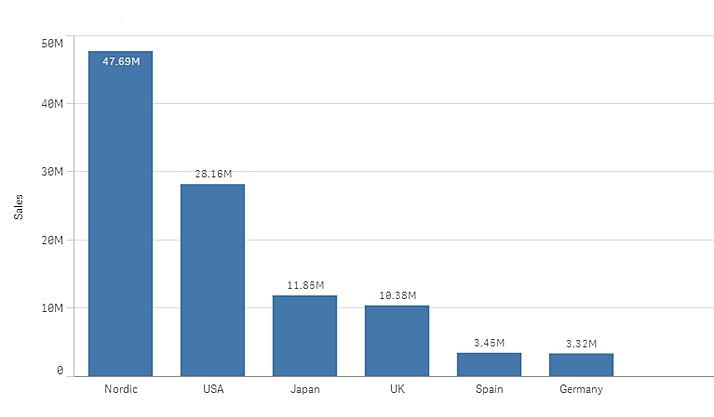
\includegraphics[width=0.25\textwidth]{grafico}
\label{fig:refejem1}
\end{figure}
 
Como puede ver en la figura \ref{fig:refejem1}, en la P.# \pageref{fig:refejem1}.
\end{lstlisting}

Las referencias una vez compiladas se ven como:
\begin{figure}[H]
    \centering
    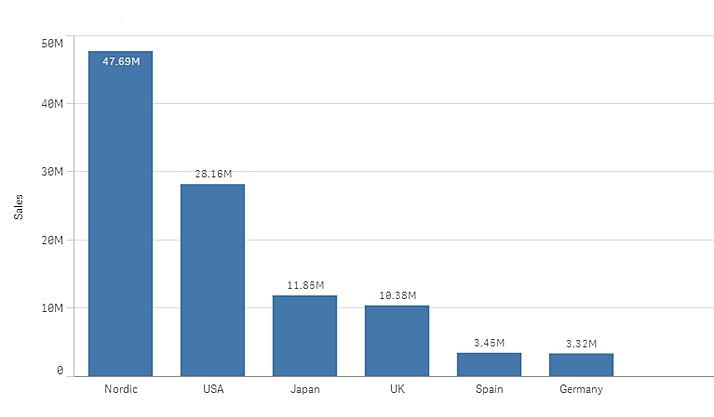
\includegraphics[width=0.25\textwidth]{grafico}
    \caption{refejem1}
    \label{fig:refejem1}
\end{figure}
 
Como puede ver en la figura \ref{fig:refejem1} en la P.\# \pageref{fig:refejem1}.

\section{Manejo de figuras al lado de tablas (minipage)}
El minipage es una funcionalidad de \LaTeX{} utilizada para poner lado a lado estructuras que de otra forma ser\'{\i}a dif\'{\i}cil, su armaz\'{o}n en c\'{o}digo se ve como:

\begin{lstlisting}
\begin{minipage}[ajuste]{ancho del minipage}
  Texto ... \ \
  Imagenes ... \ \
  Tablas ... \ \
\end{minipage} 
\end{lstlisting}

Partiendo de esta implementaci\'{o}n se pueden crear diferentes configuraciones.

Ejemplo de tabla + tabla.

\begin{lstlisting}
\begin{minipage}{0.2\textwidth}
\begin{tabular}{|c|c|c|}
\hline
 A & B & C \\
\hline
 1 & 2 & 3  \\
\hline 
 4 & 5 & 6 \\
\hline
\end{tabular}
\end{minipage}
\begin{minipage}{0.2\textwidth}
\begin{tabular}{c|c|c}
 A & B & C \\
\hline
 1 & 2 & 3  \\
\hline 
 4 & 5 & 6 \\
\end{tabular}
\end{minipage}
\end{lstlisting}

\begin{minipage}{0.2\textwidth}
\begin{tabular}{|c|c|c|}
\hline
 A & B & C \\
\hline
 1 & 2 & 3  \\
\hline 
 4 & 5 & 6 \\
\hline
\end{tabular}
\end{minipage}
\begin{minipage}{0.2\textwidth}
\begin{tabular}{c|c|c}
 A & B & C \\
\hline
 1 & 2 & 3  \\
\hline 
 4 & 5 & 6 \\
\end{tabular}
\end{minipage}
\\
\\
Ejemplo de imagen + texto.

\begin{lstlisting}
\begin{minipage}[t]{0.2\textwidth}

\includegraphics[scale=0.4]{tec-logo}
\end{minipage}
\begin{minipage}{0.2\textwidth}
Tecnologico de CR\\
Tecnologico de CR\\
Tecnologico de CR\\
Tecnologico de CR\\
Tecnologico de CR\\
\end{minipage}
\end{lstlisting}

\begin{minipage}[t]{0.2\textwidth}

\includegraphics[scale=0.4]{tec-logo}
\end{minipage}
\begin{minipage}{0.2\textwidth}
Tecnol\'{o}gico de CR\\
Tecnol\'{o}gico de CR\\
Tecnol\'{o}gico de CR\\
Tecnol\'{o}gico de CR\\
Tecnol\'{o}gico de CR\\
\end{minipage}

Ejemplos de imagen + imagen + imagen.

\begin{lstlisting}
\begin{minipage}[b]{0.15\textwidth}

\includegraphics[width=\textwidth]{tec-logo}
\end{minipage}
\begin{minipage}[t]{0.15\textwidth}

\includegraphics[width=\textwidth]{tec-logo}
\end{minipage}
\begin{minipage}[t]{0.15\textwidth}

\includegraphics[width=\textwidth]{tec-logo}
\end{minipage}
\end{lstlisting}

\begin{minipage}[b]{0.15\textwidth}

\includegraphics[width=\textwidth]{tec-logo}
\end{minipage}
\begin{minipage}[t]{0.15\textwidth}

\includegraphics[width=\textwidth]{tec-logo}
\end{minipage}
\begin{minipage}[t]{0.15\textwidth}

\includegraphics[width=\textwidth]{tec-logo}
\end{minipage}

\section{Ecuaciones matem\'aticas}
En este segmento se presentan las caracter\'{\i}sticas b\'{a}sicas para generar f\'{o}rmulas matem\'{a}ticas en \LaTeX{}.

\subsection{Modo matem\'{a}ticas}
\LaTeX{} permite dos tipos de f\'{o}rmulas: inline y display, la primera permite escribir la f\'{o}rmula en l\'{\i}nea con el texto y la segunda lo opuesto, por lo que cuando se escriba ocupar\'{a} una l\'{\i}nea completa por si sola.\par
Las f\'{o}rmulas \textquotedblleft{}inline\textquotedblright{} se caracterizan por estar delimitadas por \textdollar{}formula\textdollar{} y las \textquotedblleft{}display\textquotedblright{} por \textdollar{}\textdollar{}formula\textdollar{}\textdollar{} o \textbackslash{}begin\{equation\} formula \textbackslash{}end\{equation\}. Cabe recalcar que en el modo inline las expresiones son compresas para seguir con la l\'{\i}nea del texto.

Ejemplo de inline:

\begin{lstlisting}
La formula $E=MC^2$ fue formulada por Einstein anos despues de presentar su teoria de la relativadad.
\end{lstlisting}

La f\'{o}rmula $E=MC^2$ fue formulada por Einstein a\~{n}os despu\'{e}s de presentar su teor\'{i}a de la relativadad.

Ejemplo de display:
\begin{lstlisting}
La formula $$E=MC^2$$ fue formulada por Einstein anos despues de presentar su teoria de la relativadad.En unidades naturales ($c$ = 1), representa la identidad

\begin{equation}
E = m
\end{equation}
\end{lstlisting}
La f\'{o}rmula $$E=MC^2$$ fue formulada por Einstein a\~{n}os despu\'{e}s de presentar su teor\'{i}a de la relativadad.En unidades naturales ($c$ = 1), representa la identidad

\begin{equation}
E = m
\end{equation}

\subsection{S\'{i}mbolos especiales}
La utilizaci\'{o}n de s\'{\i}mbolos especiales se da por el modo matem\'{a}tica explicado en el punto anterior, solamente basta escribir \textbackslash{}simbolo dentro de los \textdollar{} \textdollar{}.

\begin{lstlisting}
$$\delta \alpha$$
\end{lstlisting}

$$\delta \alpha$$

\subsection{Fracciones}

Las fracciones pueden ser utilizadas en conjunto con el texto $\frac{1}{2} $ o por si solas con los modos inline y display.

$$\frac{1}{2} $$

Las fracciones son muy vers\'{a}tiles, pudiendo ser anidadas para expresiones complejas.

\begin{lstlisting}
Ejemplo sencillo:

$$\frac{1}{2}$$

Ejemplo anidado:
 
$$ \frac{1+\frac{a}{b}}{1+\frac{1}{1+\frac{1}{a}}} $$
 
\end{lstlisting}

Ejemplo sencillo:

$$\frac{1}{2}$$

Ejemplo anidado:
 
$$ \frac{1+\frac{a}{b}}{1+\frac{1}{1+\frac{1}{a}}} $$
 
\subsection{Operadores}
El manejo de operadores es muy variado por lo que a continuaci\'{o}n se explican los m\'{a}s utilizados.

$$\int_{a}^{b} x^2 dx$$

Las integrales como la anterior son definidas en \LaTeX{} como:

\begin{lstlisting}
\int_{superior}^{inferior}

$$\int_{a}^{b} x^2 dx$$
\end{lstlisting}

Integrales anidadas pueden resultar m\'as complejas, pero se pueden obtener modificando el inicio de la expresi\'on (int) como en los siguientes ejemplos:
\begin{lstlisting}
$$\iint_V \mu(u,v) \,du\,dv$$
$$\iiint_V \mu(u,v,w) \,du\,dv\,dw$$
$$\idotsint_V \mu(u_1,\dots,u_k) \,du_1 \dots du_k$$
\end{lstlisting}

$$\iint_V \mu(u,v) \,du\,dv$$
$$\iiint_V \mu(u,v,w) \,du\,dv\,dw$$
$$\idotsint_V \mu(u_1,\dots,u_k) \,du_1 \dots du_k$$

Al igual que las integrales, las sumatorias est\'{a}n dadas por:
\begin{lstlisting}
\sum_{superior}^{inferior}

Ejemplo:
Sum $\sum_{n=1}^{\infty} 2^{-n} = 1$ inside text
\end{lstlisting}

$$\sum_{n=1}^{\infty} 2^{-n} = 1$$

En el caso de los l\'{i}mites se utiliza el comando

\begin{lstlisting}
\lim_{lower}

Ejemplo:
$$\lim_{x\to\infty} f(x)$$
\end{lstlisting}

$$\lim_{x\to\infty} f(x)$$

\section{Manejo de colores}
El manejo de colores en \LaTeX{} est\'{a} dado por los paquetes

\begin{lstlisting}
\usepackage{color}
\usepackage{xcolor}
\end{lstlisting}

Ambos paquetes permiten de colores predefinidos, pero a la vez tiene la flexibilidad de modificar los colores y secciones a gusto. El siguiente ejemplo muestra los colores predefinidos.

\begin{lstlisting}
\begin{itemize}
\color{blue}
\item Primer item
\item Segundo item
\end{itemize}
 
\noindent
{\color{red} \rule{\linewidth}{0.5mm} }
\end{lstlisting}

\begin{itemize}
\color{blue}
\item Primer item
\item Segundo item
\end{itemize}
 
\noindent
{\color{red} \rule{\linewidth}{0.5mm} }

Los colores red y blue est\'{a} predefinidos en el paquete color, algunos otros ejemplos b\'{a}sicos son.

\begin{lstlisting}
El color del texto puede ser cambiado a \textcolor{red}{rojo}. Tambien puede cambiar el background del \colorbox{BurntOrange}{texto}.
\end{lstlisting}

El color del texto puede ser cambiado a \textcolor{red}{rojo}. Tambien puede cambiar el background del \colorbox{orange}{texto}.\par{}

Para una mayor variedad de colores se pueden crear variables de color d\'{a}ndole una etiqueta a un valor RGB.

\begin{lstlisting}
\definecolor{rosado}{rgb}{0.858, 0.188, 0.478}
\definecolor{gris}{gray}{0.6}
\end{lstlisting}

\definecolor{rosado}{rgb}{0.858, 0.188, 0.478}
\definecolor{gris}{gray}{0.6}

\begin{enumerate}
\item \textcolor{rosado}{Rosado}
\item \textcolor{gris}{Gris}
\end{enumerate}

El definecolor utiliza una de las siguientes 4 opciones para el primer par\'{a}metro.

\begin{enumerate}
\item \textbf{rgb}: rojo, verde, azul. Tres valores separados por comas entre 0 y 1 definen los componentes del color.
\item \textbf{RGB}: lo mismo que rgb, pero los n\'{u}meros son enteros entre 0 y 255.
\item \textbf{cmyk}: cian, magenta, amarillo y blacK. Lista de cuatro n\'{u}meros separados por comas entre 0 y 1 que determina el color de acuerdo con el modelo aditivo utilizado en la mayor\'{\i}a de las impresoras.
\item \textbf{gray}: escala de grises. Un solo n\'{u}mero entre 0 y 1.
\end{enumerate}

Adem\'{a} de modificar el color del texto se puede cambiar el color de la p\'{a}gina con

\begin{lstlisting}
\pagecolor{black}
\end{lstlisting}


\includegraphics[scale=1]{ejemplofondo}

\begin{thebibliography}{1}
\bibitem{[1]}The Editors of Encyclopaedia Britannica  (2013) \emph{LaTeX COMPUTER PROGRAMMING LANGUAGE} [Blog post]. Consultado desde https://www.britannica.com/technology/LaTeX-computer-programming-language
\bibitem{[2]} \emph{Introduction to LaTeX.} (2018). Consultado desde https://www.latex-project.org/about/
\bibitem{[3]} \emph{Basic description of file types and how LaTeX works.} (2018). Consultado desde http://personal.bgsu.edu/~zirbel/5920/latex/latex\_basics.htm
\bibitem{a} \emph{Latex-Tutorial.} (2018). Consultado desde https://www.latex-tutorial.com
\bibitem{b} \emph{ShareLatex.} (2018). Consultado desde https://www.sharelatex.com/learn
\bibitem{c} \emph{Sascha-Frank.} (2018). Consultado desde http://www.sascha-frank.com
\bibitem{[7]} \emph{Alineación de párrafos.} (2018). Consultado desde https://latextips.wordpress.com/2009/01/27/alineacion-de-parrafos/

\end{thebibliography}
\end{document}






